% Using KOMA Script document style
% Font size setting and
% option to skip empty lines as new paragraphs
\documentclass[10pt,a4paper]{article}
% Packages without Options
\usepackage{
	algorithm,
	alltt,
	algpseudocode,
	amsfonts,
	amssymb,
	appendix,
	array,
	booktabs,
	dirtree,
	enumitem,
	float,
	footnote,
	gensymb,
	geometry,
	graphicx,
	interval,
	karnaugh-map,
	lipsum,
	listings,
	longtable,
	makecell,
	mathtools,
	minted,
  nicematrix,
	parskip,
	pdfpages,
	pgfkeys,
	pgfplots,
	subcaption,
	tabularx,
	tablefootnote,
	textcomp,
	tikz,
    titlecaps,
	venndiagram,
	wrapfig,
	wrapfig,
	xcolor
}



% Packages with Options

\usepackage[framemethod=tikz]{mdframed}
\usepackage[colorlinks,linkcolor=cyan, citecolor=cyan, urlcolor=cyan]{hyperref}
\usepackage[labelfont=bf,textfont=it,labelsep=period]{caption}
\usepackage[RPvoltages]{circuitikz}
\usepackage[english]{babel}
\usepackage[nameinlink,noabbrev]{cleveref}

\definecolor{mintedbackground}{rgb}{0.97,0.97,0.97}

\setminted[cpp]{
bgcolor=mintedbackground,
    linenos=true,
    breaklines=true,}

\setminted[js]{
bgcolor=mintedbackground,
    linenos=true,
    breaklines=true,}

\setminted[python]{
bgcolor=mintedbackground,
    linenos=true,
    breaklines=true,}
    

\linespread{1.5}

% Package: AlgorithmicX
% Sets all comments to be indentend and aligned

\renewcommand{\Comment}[2][.7\linewidth]{%
  \leavevmode\hfill\makebox[#1][l]{//~#2}}


% Package: Interval
% Sets the style of mathematical intervals
\intervalconfig{
soft open fences, separator symbol=,,
}

% Package: Geometry
% Sets the page margins
\geometry{
    a4paper,
    left=32mm,
    right=22mm,
    top=22mm,
    }
	
% Creates a proper caption name for algorithms
\newcommand{\algorithmautorefname}{Algorithm}
\newcommand{\listingautorefname}{Listing}
\algrenewcommand{\algorithmiccomment}[1]{\texttt{// #1} }
% Creates a numbered environment for Theorems
\newtheorem{theorem}{Theorem}

% Redefine the implication arrow to be a simple, thin arrow instead of the default, thick arrow
\renewcommand{\implies}{\rightarrow}

% Create a new command for the set complement to make my logical statements easier to read
\newcommand{\compl}{\overline}

% Creates commands for combinatorics nCr and nPr
\newcommand{\nCr}[2]{\,_{#1}C_{#2}} % nCr
\newcommand{\nPr}[2]{\,_{#1}P_{#2}} % nPr

% Package: tikz
% Loads libraries for drawing automata, 
\usetikzlibrary{automata,positioning,shadows,arrows, shapes.gates.logic.US, calc}

% Creates a command to create a button shape
\newcommand*\keystroke[1]{%
  \tikz[baseline= (key.base)]
    \node[%
      draw,
      fill=white,
      drop shadow={shadow xshift=0.25ex,shadow yshift=-0.25ex,fill=black,opacity=0.75},
      rectangle,
      rounded corners=2pt,
      inner sep=1pt,
      line width=0.5pt,
      font=\scriptsize\sffamily
    ] (key) {#1\strut};
}

% Package: pgfplot
% Sets the global options for PGF Plots
\pgfplotsset{compat=newest}

% Package: tikz
% Flowchart Shapes
\tikzstyle{startstop} = [rectangle, rounded corners, minimum width=3cm, minimum height=1cm,text centered, draw=black, fill=red!30]
\tikzstyle{io} = [trapezium, trapezium left angle=70, trapezium right angle=110, minimum width=3cm, minimum height=1cm, text centered, draw=black, fill=blue!30]
\tikzstyle{process} = [rectangle, minimum width=3cm, minimum height=1cm, text centered, draw=black, fill=orange!30]
\tikzstyle{decision} = [diamond, minimum width=3cm, minimum height=1cm, text centered, draw=black, fill=green!30]
\tikzstyle{arrow} = [thick,->,>=stealth]

% Disable Minted syntax error highlights (red boxes)
\AtBeginEnvironment{minted}{%
  \renewcommand{\fcolorbox}[4][]{#4}}

% Listings Style (non-minted)

\lstdefinestyle{arjuncode}{
    basicstyle=\ttfamily,
    breakatwhitespace=false,         
    breaklines=true,                 
    captionpos=b,                    
    keepspaces=true,                 
    numbers=left,                    
    numbersep=5pt,                  
    showspaces=false,                
    showstringspaces=false,
    showtabs=false,                  
    tabsize=2
}

\lstset{style=arjuncode}

\graphicspath{{images/}}

 %Adjust this based on where your Summary is stored
\title{CM3015: Machine Learning \& Neural Networks \\ Summary}
\author{Arjun Muralidharan}
\begin{document}

\maketitle
\newpage
\tableofcontents
\listoffigures
\listoftables
% \listofalgorithms

\newpage
\renewcommand{\subsubsectionautorefname}{section\negthinspace}

\section{Introduction to Machine Learning and Neural Networks}
\begin{mdframed}
\textbf{Learning Outcomes}
\begin{itemize}[label={\checkmark}]
\item Explain fundamental machine learning concepts
\item Describe various types of machine learning problem
\item Describe various applications of machine learning
\end{itemize}
\end{mdframed}

\subsection{Types of Machine Learning}

In most cases where machine learning is used, we don't know what the actual problem is. There are two types of ML problems.

\paragraph{Supervised learning} The agent observes input-output pairs and learns a \textit{function} that maps from input to output. The outputs (``answers'') provided are called \textbf{labels}.

Given a training set of \(N\) example input-output pairs
\[
(x_1, y_1),(x_2, y_2),...(x_n, y_n)
\]

where each pair was generated by an unknown function \(y = f(x)\), discover a function \(h\) that approximates the true function \(f\), stated as 
\[
h(x) \rightarrow y    
\]


Essentially, we provide the ``answers'' to the problem as inputs, and the AI system comes up with the ``rules''.

The outputs can be \textbf{discrete}, for example a classification into a specific group, or \textbf{continuous}, for example predicting a specific price.

\paragraph{Unsupervised learning} The agent only receives data but no labels, and is tasked with finding meaningful representations of the data with a variety of techniques.

\paragraph{textbf}{Reinforcement learning} The agent gets a reward for completing a desired outcome, making the agent better over time.

\subsubsection{Types of algorithms}

Depending on the problem, different algorithms are suitable to be used by an agent.

\paragraph{Regression} When predicting a continuous variable.

\paragraph{Classification} When predicting a discrete output, such as assigning data to groups.

\paragraph{Clustering} When identifying new groupings of data in an unsupervised scenario.

\subsection{Machine Learning Black Box}

A typical machine learning pipeline involves taking a set of \textbf{labels} \(Y\) and a set of \textbf{data} \(X\), which the agent processes into a \textbf{mapping} of \(X\) to \(Y\). This mapping can then be used to map new data to a prediction.

Within the agent, data is often taken through \textbf{feature pre-processing} before reaching the ML algorithm, which is fed with the labels.

\subsection{Deep Learning}

A subset of ML, \textbf{deep learning} is an approach to learning representations from data that puts an emphasis on learning \textit{successive layers} of increasingly meaningful representations.

In deep learning, these layered representations are (almost always) learned via models called \textit{neural networks}.

\begin{figure}[h]
    \centering
    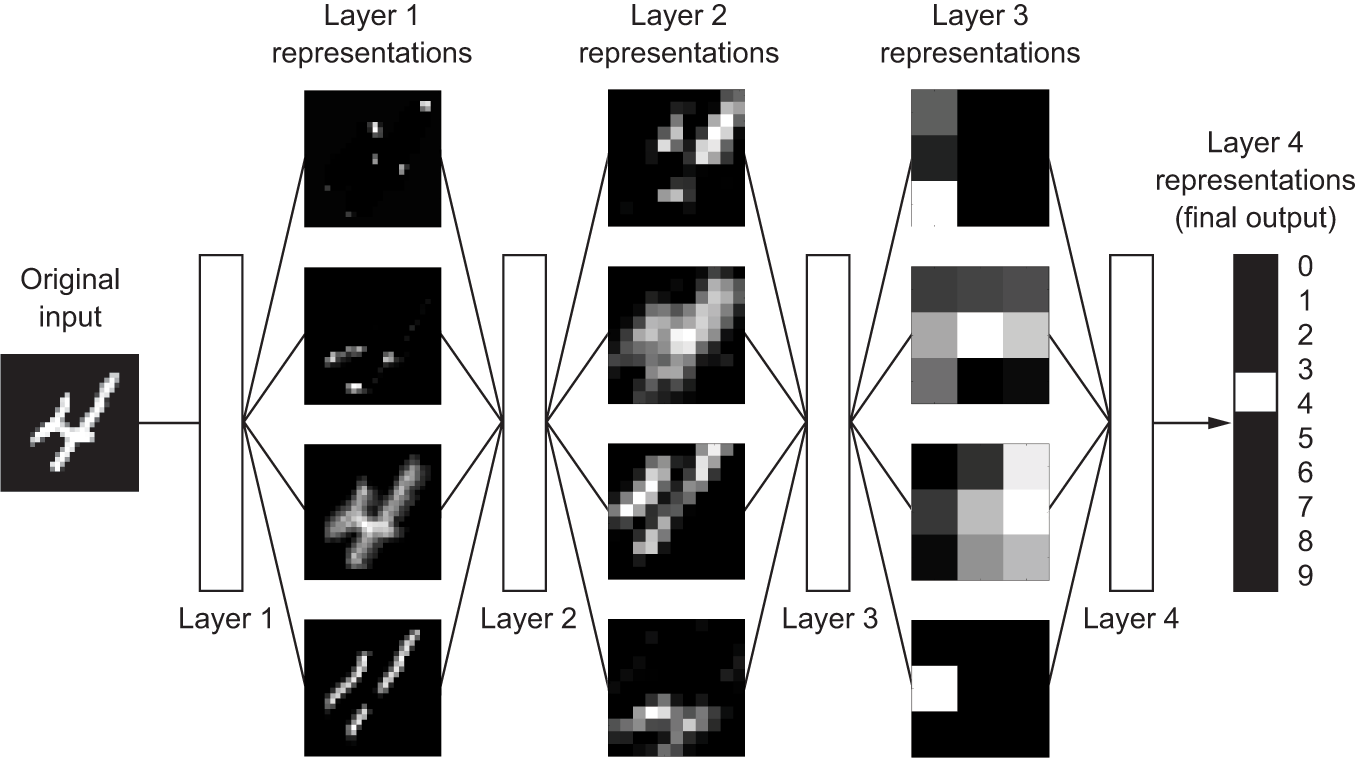
\includegraphics[width=7cm]{dl}
    \caption{Deep learning representation}
    \label{fig:dl}
\end{figure}

The specification of what each layer does is encoded in \textit{weights}, also called the \textit{parametrization} of the layers. These are initially assigned at random.

The \textbf{loss function} or cost function takes the predictions of the agent, compares them to the true targets and generates a \textit{loss score}.

This score is used by the \textbf{optimizer}, which implements a \textbf{Backpropagatgion algorithm} to adjust the weights and improve the model.

\end{document}

